\documentclass[11pt,a4paper]{article}
\usepackage[utf8]{inputenc}
\usepackage[T1]{fontenc}
\usepackage[margin=2.5cm]{geometry}
\usepackage{amsmath}
\usepackage{array}
\usepackage{booktabs}
\usepackage{enumitem}
\usepackage{graphicx}
\graphicspath{{figures/}}
\usepackage[hidelinks]{hyperref}

\usepackage{xurl}
\makeatletter\g@addto@macro\UrlBreaks{\do\_}\makeatother
\newcommand{\code}[1]{\path{#1}}
\newcommand{\doi}[1]{\href{https://doi.org/#1}{doi:#1}}
\newcommand{\ra}{\raggedright\arraybackslash}
\sloppy

\title{The Kanizsa saliences model against the spatiotopic, retinotopic and deflationary views of visual stability}
\author{Francesco Mannella}
\date{October 7, 2026 \\ \small branch \code{saliencies}; working note}

\begin{document}
\maketitle

\begin{abstract}
\noindent
The draft presents the model as an account of visual stability and anticipatory
remapping (Figure~1 of the draft). This note compares it with the three views
organised in \code{docs/visual_stability_review.tex}: spatiotopic, retinotopic
remapping and deflationary. It reads what the model implements from the code, sets
what the draft claims against what the code does, and collects evidence for and
against the model from the project's own results and from the literature. The
model is closest to a contingency-based account of stability, and only partly
an account of remapping: its anticipation is an address on a lattice, not a shift
of receptive fields, and the anticipated effect is not read out at run time.
Stability across starting positions has not been tested. A map-level
predictive-remapping paradigm on wider-window runs finds future-field responses no more
than a shuffled-pairing control does, and the maps show indirect retinotopy in a
black-box probe.
\end{abstract}

\section{Scope and sources}

\begin{itemize}[nosep]
  \item \textbf{The claim under test.} \code{docs/draft.tex}: the abstract (l.62--76)
    describes visual stability as ``the alignment of motor commands and resultant
    sensory inputs'', with retinal states that ``anticipate effects and initiate
    saccades'', ``confirmation of congruence between saccades and visual outcomes'',
    and no need for feedback correction; the stub on neural substrates lists
    remapping of FEF and LIP receptive fields. Figure~1 of the draft
    (\code{docs/figures/meccanism.png}, caption still empty) illustrates the mechanism.
  \item \textbf{The model.} \code{src/model/*.py}, read directly; results from
    \code{docs/report.tex} and from the probe of \code{docs/topological_stability.tex}.
  \item \textbf{The views.} The review \code{docs/visual_stability_review.tex}.
\end{itemize}

\section{The model as the draft depicts it}

\begin{figure}[h]
\centering
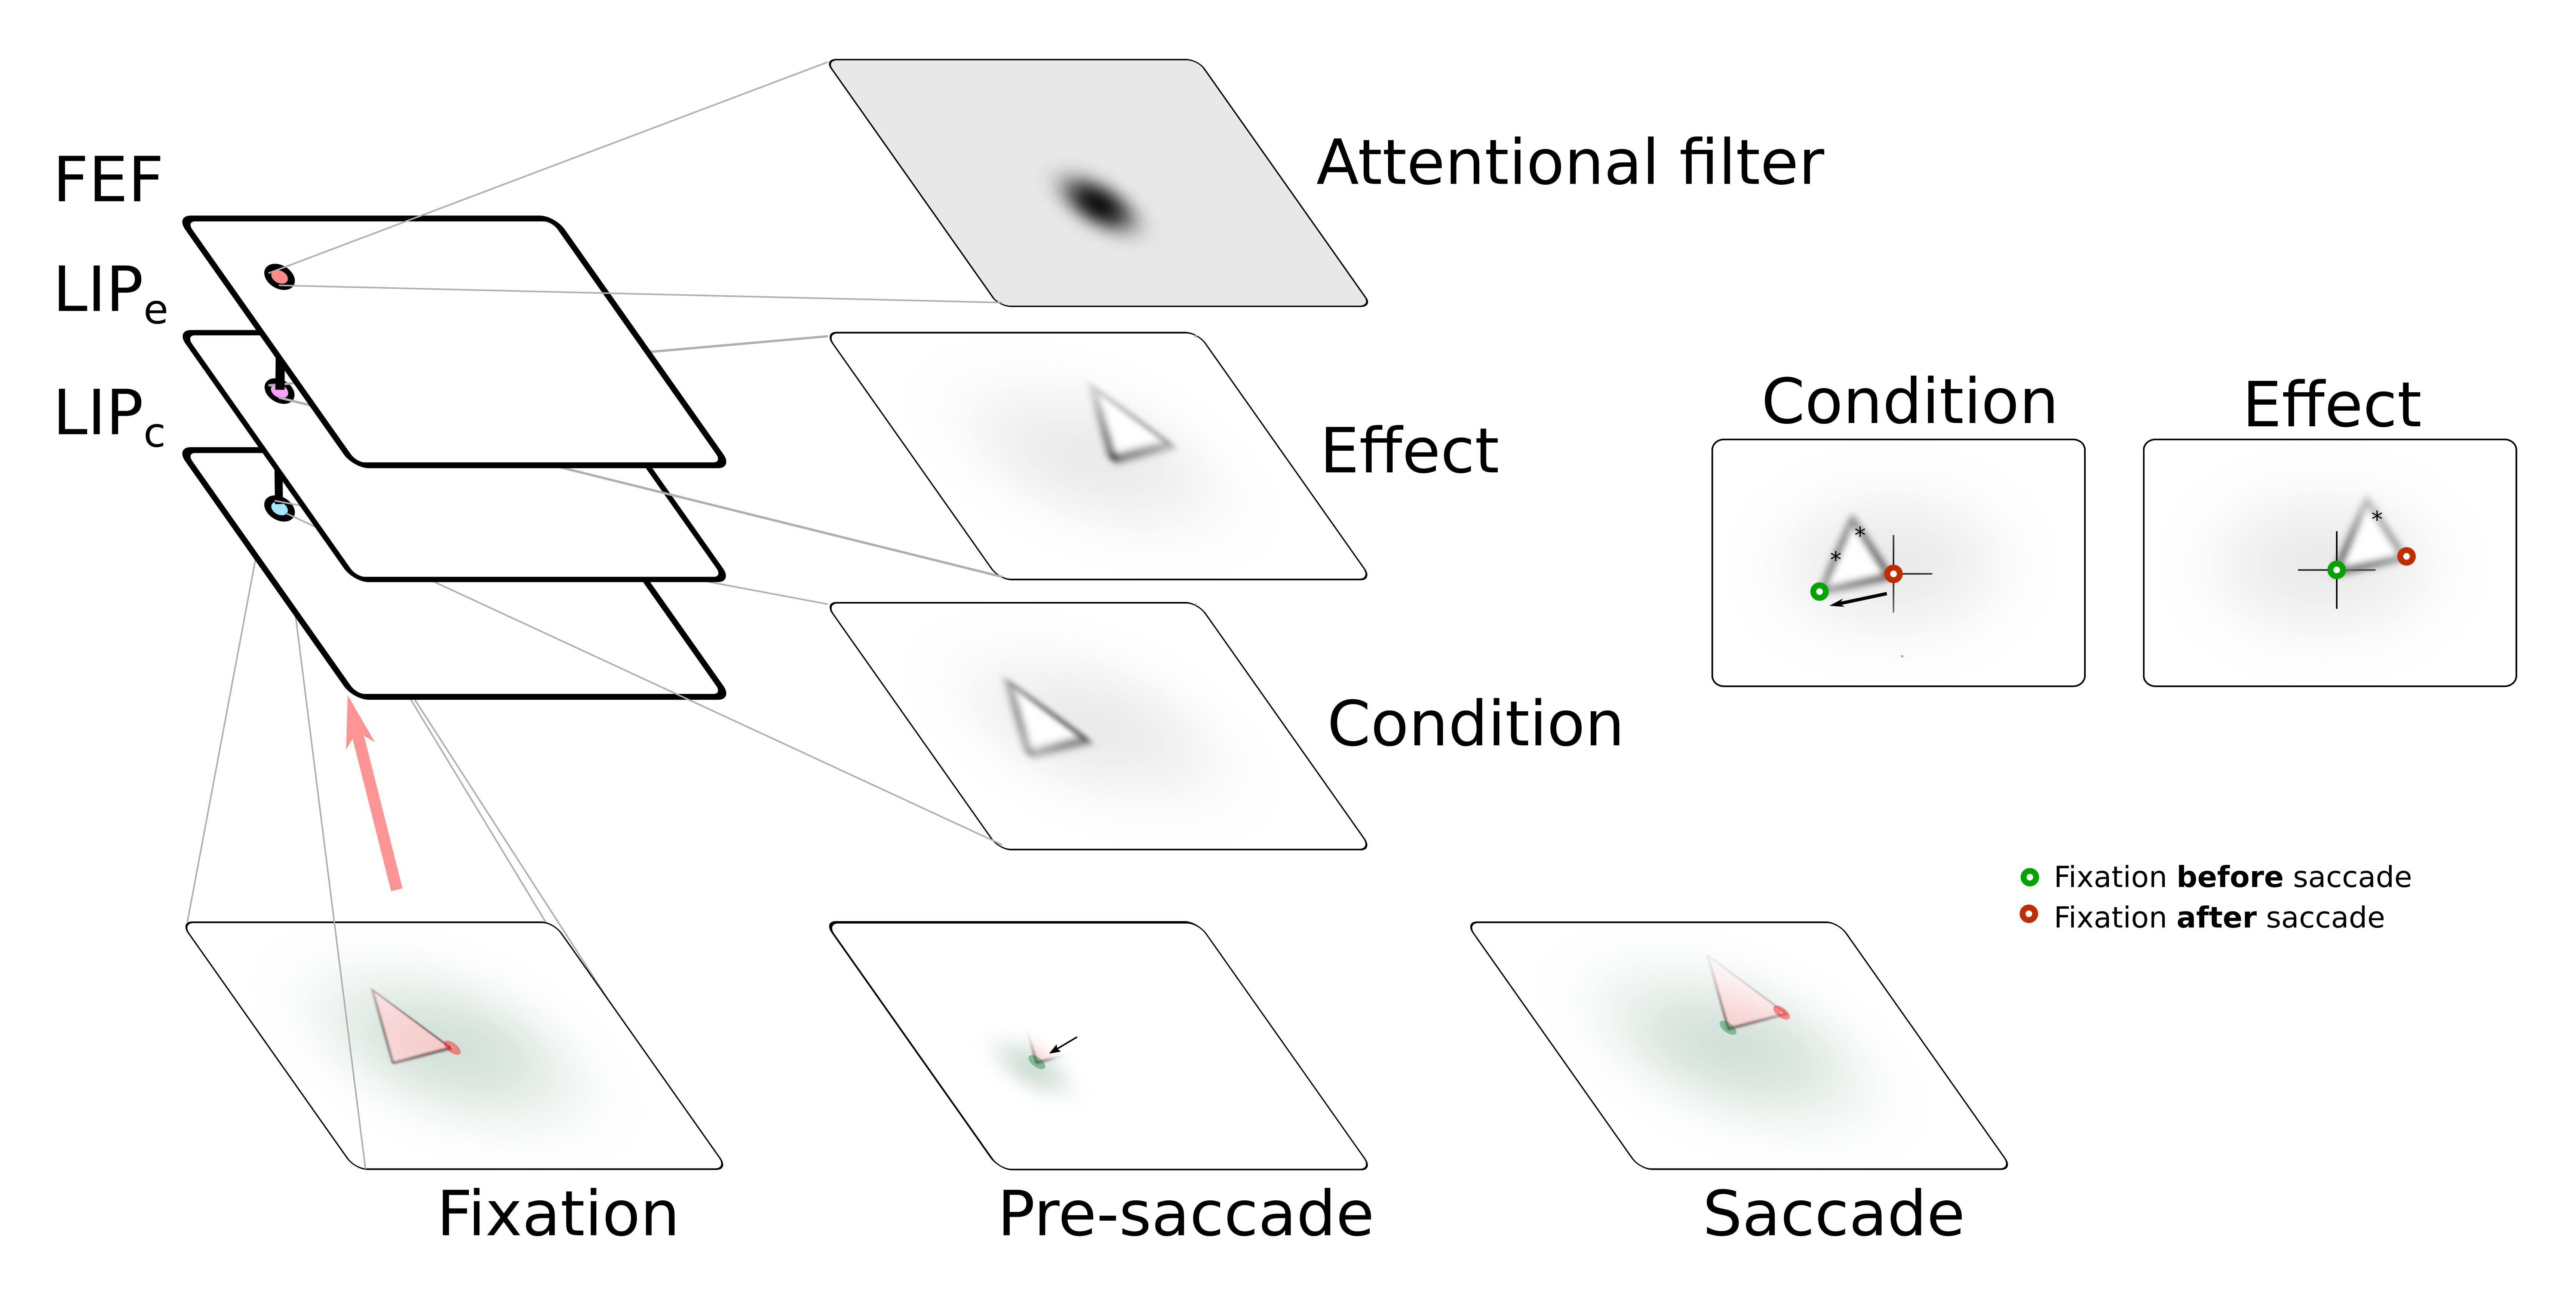
\includegraphics[width=0.85\textwidth]{meccanism.png}
\caption{The draft's mechanism figure (\texttt{meccanism.png}). The caption is
empty in the draft; this is our reading. Left: three stacked layers, FEF with an
attentional filter, LIP$_\mathrm{e}$ (effect) and LIP$_\mathrm{c}$ (condition),
linked unit by unit. The bottom row shows fixation (the retinal view feeds the
condition layer, pink arrow), the pre-saccadic state (a narrowed attentional focus
and the saccade vector) and the saccade. Right: the condition is the view before the
saccade (green fixation), the effect is the view after it (red fixation).}
\end{figure}

The figure shows a column of units, one per lattice position, that spans three
layers: a condition (the foveal view before the saccade), an effect (the view after
it) and an attentional filter that selects the saccade. The draft reads these as LIP
and FEF populations: LIP$_\mathrm{c}$ holds the condition, LIP$_\mathrm{e}$ the
anticipated effect, and FEF the attentional filter that drives the saccade. The
retinal view reaches the condition layer; within one column the same unit pattern
addresses the effect and the saccade. This is the draft's account of both
phenomena: \emph{stability} is the congruence of the anticipated effect with the
actual one, and \emph{anticipatory remapping} is that the effect layer is
activated by the condition before the saccade.

\begin{table}[h]
\centering\footnotesize
\setlength{\tabcolsep}{3pt}
\begin{tabular}{@{}>{\ra}p{3.4cm}>{\ra}p{4.0cm}>{\ra}p{3.6cm}>{\ra}p{3.9cm}@{}}
\toprule
Element in the draft's figure & Implementation & Location & Caveat \\
\midrule
LIP$_\mathrm{c}$, condition & \code{visual_conditions_map}: topographic map of the $16\times16$ colour-saliency fovea before the saccade & \code{offline_controller.py} l.95--111 & Naming as LIP is the draft's hypothesis \\
LIP$_\mathrm{e}$, effect & \code{visual_effects_map}: same map type, trained on the fovea two steps after the saccade & \code{offline_controller.py} l.109 & Used only in training and in the match (below) \\
FEF, attentional filter & \code{attention_map}: map of the retina-normalised attention centre; the saccade is its prototype at the goal cell & \code{offline_controller.py} l.291 & Action space is retinal-vector \\
Link between layers & One anchor, the goal cell (the conditions winner), aligns the three maps (STM loss) & \code{offline_controller.py} l.491; \code{topological_maps.py} l.326--365 & Alignment is learned offline \\
Retinal feed to LIP$_\mathrm{c}$ & Fovea crop of the saliency map & \code{agent.py} l.221 & Retina-centred input \\
Attentional filter & Gaussian mask over the saliency map & \code{agent.py} l.55, l.164 & Reset to the retina centre after each decision \\
\bottomrule
\end{tabular}
\caption{Draft figure against code.}
\label{tab:fig}
\end{table}

\section{Anticipatory remapping in the model: what is implemented}

Three facts from the code bound the claim.

\begin{enumerate}[nosep]
  \item \textbf{The anticipation is an address.} The goal cell addresses a condition
    prototype, an attention prototype (the saccade) and an effect prototype (the
    expected post-saccadic view) at once. The effect prototype is the stored
    expectation, a lookup, not a computed prediction of the image.
  \item \textbf{The expected effect is not read out at run time.} The effects map is
    used only in the offline update and in the match that defines competence
    (\code{offline_controller.py} l.482, l.510, l.547). At decision time the model
    reads the conditions winner and the attention prototype at that cell
    (\code{generate_saccade}, l.291; \code{get_action_from_condition}, l.671);
    \code{test.py} never calls the effects map. So the ``confirmation of congruence''
    of the draft is computed during training, not as a comparison at run time.
  \item \textbf{No receptive field moves.} Maps are fixed during a saccade and change
    only in the epoch update (l.369). The model does not shift receptive fields
    toward the saccade target and has no pre-saccadic response at a future field,
    the signatures reported in LIP and FEF (Duhamel et al., 1992; Zirnsak et al.,
    2014). The draft's neural-substrates stub lists remapping of FEF and LIP
    receptive fields, which the model does not reproduce.
\end{enumerate}

In the draft's terms the model therefore gives the \emph{functional} counterpart
of remapping, a learned relation between a view, a saccade and its effect, and not
its neural signatures. Whether that relation could produce the signatures is
open (Section~\ref{sec:tests}).

\section{Comparison with the three views}

\begin{table}[h]
\centering\footnotesize
\setlength{\tabcolsep}{3pt}
\begin{tabular}{@{}>{\ra}p{2.2cm}>{\ra}p{2.7cm}>{\ra}p{2.7cm}>{\ra}p{2.7cm}>{\ra}p{3.2cm}@{}}
\toprule
& Spatiotopic & Retinotopic remapping & Deflationary & The model \\
\midrule
Frame & World or head & Eye & None needed & Lattice of aligned maps; inputs and actions retina-centred \\
What is carried & Position in external coordinates & Retinal activity or pointers at the new location & Little; the scene is re-sampled & Condition--action--effect triples \\
Update signal & Eye position & Corollary discharge & Not central & Anchor, written by the selected action \\
Predictive model & Eye-position signal & Where items will land & Contingency knowledge & Lookup on a lattice; no image prediction \\
Anticipatory remapping & Not required & Shift of receptive fields or pointers before the eye lands & Not needed & Effect prototype addressed before the saccade; not read out \\
Stability criterion & Map in external coordinates & Continuous updating & Assumed stability, post-saccadic landmarks & Congruence of effect with expectation, in training \\
\bottomrule
\end{tabular}
\caption{The model against the three views.}
\label{tab:views}
\end{table}

\subsection{Against spatiotopy}

\emph{Agreement.} None on mechanism. The model has no world-centred map, no
eye-position signal (absolute eye position stays inside the environment), and
needs neither for its behaviour. It agrees only in the observation that
spatiotopic neurons are a minority and that eye-position signals are unreliable
after a saccade (Xu et al., 2012; Morris et al., 2012), which removes a motive for
a global frame.

\emph{Disagreement.} The model is silent on the spatiotopic evidence: the positional
motion aftereffect (Turi and Burr, 2012), the fMRI repetition suppression across a
saccade (Fairhall et al., 2017) and spatiotopic updating within 150~ms (Fabius et
al., 2019). These tests oppose the frames by a saccade; the model was never run on
such a paradigm. Either it must reproduce the spatiotopic pattern from address
lookups, or it predicts the effects away.

\subsection{Against retinotopic remapping}

\emph{Agreement.} The model uses an action-derived signal (the anchor) and an
anticipated effect, and it names FEF and LIP, the areas where remapping is
reported. It also keeps retina-centred inputs and actions. The draft's abstract
describes the model as taking ``a retinotopic updating perspective'' (l.64).

\emph{Disagreement.} Remapping accounts shift activity or pointers to the
post-saccadic location before the eye lands, and need a signal that says where each
item will land. The model has neither: no receptive field moves, the effect is a
learned lookup, and nothing computes a landing position. The anchor resembles a
corollary discharge, but it addresses a lattice cell, not a retinal displacement.
The draft's framing as ``retinotopic updating'' and the topological reading in
\code{docs/topological_stability.tex} point in different directions, and the draft
sentence would have to change.

\subsection{Against the deflationary view}

\emph{Agreement.} This is the closest view. The model stores condition--action--effect
triples, which is the learned relation between movement and sensory change that the
sensorimotor account calls mastery of contingencies (O'Regan and No\"e, 2001), it
has no predictive model of space, and its stability needs no feedback correction.
The failures found, in which the effect is not the effect of the addressed saccade
(reversals), are the failures a contingency account predicts.

\emph{Disagreement.} The sensorimotor account denies internal representations of
the scene, whereas the model stores explicit prototype maps and a goal cell. It also
does not use post-saccadic landmarks or the suppression of displacement
(Bridgeman et al., 1975; Deubel et al., 1996), and it does not explain why displacements
are undetected during saccades.

\section{Evidence for the model}

Strength: \emph{direct} means the result tests the claim; \emph{indirect} that it is
consistent with it; \emph{weak} that it is suggestive.

\begin{table}[h]
\centering\footnotesize
\setlength{\tabcolsep}{3pt}
\begin{tabular}{@{}>{\ra}p{4.3cm}>{\ra}p{6.1cm}>{\ra}p{1.7cm}>{\ra}p{2.8cm}@{}}
\toprule
Claim & Evidence & Strength & Source \\
\midrule
The aligned maps are ordered and competent
  & Spearman 0.89 on the conditions map, competence 0.778, attention-map topographic
    error 0.07 (\code{anchor_std} 4, baseline 0.5; three seeds)
  & Direct, for the learning mechanism
  & \code{docs/report.tex} l.286 \\
The model produces voluntary scanpaths organised by object region
  & kNN purity about 0.93 with 2.4 goals per test (reference); scanpaths separate
    object regions
  & Indirect
  & \code{docs/report.tex}, tables on scanpaths \\
Stability requires pairing the address with its real effect
  & When the attention mask resets to a nearly flat distribution, 0.426 of goal
    saccades are undone (0.331 with goal inhibition); with hold fixation reversals
    fall to 0.000 and orienting saccade restores goal diversity
  & Indirect
  & \code{docs/report.tex} l.376--500 \\
Retinotopy can be found without a retinotopic organisation
  & Spot probe: all 10 visual maps show significant retinotopy ($\rho$ 0.68--0.84,
    $z$ 26--41); 9 of 10 beat a shuffled-layout control (gain 0.14--0.27)
  & Indirect, for the topological reading
  & \code{docs/topological_stability.tex}, Section on the probe \\
The layout fits neural data on maps in frontoparietal cortex
  & Topographic maps in human frontal and parietal cortex; macaque retinotopy beyond
    classic areas
  & Weak
  & Silver and Kastner (2009); Mackey et al. (2017); Arcaro and Livingstone (2017) \\
The circuit has a counterpart
  & SC to mediodorsal thalamus to FEF carries the saccade copy; FEF and LIP show
    remapping
  & Weak
  & Sommer and Wurtz (2006); Duhamel et al. (1992) \\
\bottomrule
\end{tabular}
\caption{Evidence for the model.}
\label{tab:pro}
\end{table}

\section{Evidence against, or missing}

\begin{table}[h]
\centering\footnotesize
\setlength{\tabcolsep}{3pt}
\begin{tabular}{@{}>{\ra}p{4.0cm}>{\ra}p{6.7cm}>{\ra}p{1.6cm}>{\ra}p{2.6cm}@{}}
\toprule
Problem & Detail & Kind & Source \\
\midrule
No test of stability
  & The stable-perception test, foveating the target from different starting views,
    is only proposed
  & Missing
  & \code{docs/draft.tex} l.111 \\
No remapping signature
  & No receptive-field shift, no pre-saccadic response at a future field; maps are
    fixed during the saccade. The map-level paradigm finds future-field responses no
    more than a shuffled-pairing control does (Section~\ref{sec:results})
  & Missing
  & \code{offline_controller.py} l.369 \\
The anticipated effect is not used at run time
  & The effects map enters only training and the match; congruence is not checked
    when the model acts
  & Contradicts the draft's wording
  & \code{offline_controller.py} l.482--547; \code{test.py} \\
Retinotopic and global leftovers
  & Retina-normalised action space; retina-centred fovea; global competence
    modulates learning for all samples; draft adopts a retinotopic perspective
  & Conflict with the topological reading
  & \code{agent.py} l.221, l.264; \code{draft.tex} l.64 \\
The control loop undoes goal saccades
  & Salience saccades after the reset reverse 33--43\% of goal saccades; hold fixation
    removes them but worsens scanpaths (purity 0.93 to 0.84--0.86, pairs sharing 0.17 to
    0.68)
  & Failure in the loop
  & \code{docs/report.tex} \\
Weak and noisy maps
  & Seed variance as large as many reported differences (competence $0.727\pm0.063$ for
    five seeds); 44--64\% of attention-map units never win
  & Weakness
  & \code{docs/report.tex} \\
Spatiotopic effects unaddressed
  & Spatiotopic updating within 150~ms, spatiotopic fMRI adaptation and the positional
    motion aftereffect are not simulated
  & Missing
  & Fabius et al. (2019); Fairhall et al. (2017); Turi and Burr (2012) \\
Needs action coupling
  & A yoked agent receiving the same stream reaches high alignment on energy, but the
    anchor is then not causal
  & Limit
  & \code{knowledgebase/topological\_alignment\_formalization.html} \\
Remapping data do not match a lookup
  & In FEF, receptive fields converge on the saccade target instead of shifting
    forward; remapping is transient
  & Possible conflict
  & Zirnsak et al. (2014) \\
Simple scenes and a small fovea
  & Simulated objects, a $16\times16$ fovea and episodic goals, with no natural
    scenes or multiple objects
  & Scope
  & \code{docs/report.tex}, \code{agent.py} \\
\bottomrule
\end{tabular}
\caption{Evidence against, or missing.}
\label{tab:con}
\end{table}

\section{Tests and results}
\label{sec:results}

Tests run on the trained maps since the first version of this note. Scripts are listed
in \code{SCRIPTS.md}; data are in \code{tests/} (folders named below).

\paragraph{Start-offset invariance (E1a, pilot).} \code{scripts/exp_start_offsets.py}.
The scanpath's invariance to retina start offsets was 0.78 for the model against 0.91
for a salience-only control; the pre-stated rule failed. Stability across starting
positions is therefore not shown.

\paragraph{Forward relation between paired fields (E3, pilot).}
\code{scripts/exp_predictive_field.py}. Per lattice cell, the conditions-unit and
effects-unit fields are compared with the saccade vector of the attention prototype.
The forward-direction cosine beat its shuffled null in 4 of 5 runs with the mean
readout and in 2 of 5 with peak readouts, and the shift magnitude was near zero
(slope 0.01 to 0.08). Superseded by the paradigm below.

\paragraph{Retinotopy of the maps (Phase 1).} Reported in
\code{docs/topological_stability.tex}. In 20 runs of the champion configuration
(\code{champion.md}) the black-box spot probe gives $z>3$ in 40 of 40 maps (median
$\rho$ 0.82 for conditions, 0.76 for effects), although the maps are trained on view
content only: the retinotopy is indirect.

\paragraph{Predictive-remapping paradigm at map level (Phase 2).}
\code{scripts/exp_remap_feasibility.py} and \code{scripts/exp_remapping_paradigm.py};
rules fixed in \code{predictive_remapping.md}. For each cell $j$ the post-saccadic
field (CRF) is the effects-unit field, the pre-saccadic field is the response of
column $j$ through the model's read-out path (a lattice Gaussian around the conditions
winner), and the forward-predicted future field is $\mathrm{FF}_j=\mathrm{CRF}_j+d(j)$,
with $d(j)$ the saccade vector of the attention prototype. Only cells with FF inside the
fovea window are testable. The only quantitative benchmark is Neupane et al. (2016): the
share of future-field (FF) type remapping across V4 conditions is 0.27 to 0.82. The
latency and trace figures of LIP, V3A and FEF cannot be expressed at map level (no time
axis) and are not compared.

\emph{Feasibility.} With the $16\times16$ window, saccade amplitudes of the attention
prototypes are 26 to 32 retina pixels, and the testable fraction is 0.00 to 0.02 in all 20
champion runs (rule: at least 0.30), so the paradigm cannot be run on them. With
\code{fovea_scale} 48 and 64 (three seeds each, \code{tests/wider_window_2026-10-08}) the
testable fraction is 0.32 to 0.65 and 0.68 to 0.93, and competence is comparable (0.73
to 0.81 over the last 50 epochs).

\begin{table}[h]
\centering\footnotesize
\setlength{\tabcolsep}{4pt}
\begin{tabular}{@{}llcccccc@{}}
\toprule
Window & Seed & Testable & P1 trained & P1 shuffled & FF trained & FF shuffled & FF untrained \\
\midrule
48 & 14142 & 65 & 0.18 & 0.21 & 0.37 & 0.40 & 0.00 \\
48 & 17320 & 43 & 0.47 & 0.52 & 0.60 & 0.74 & 0.07 \\
48 & 22360 & 29 & 0.14 & 0.33 & 0.48 & 0.64 & 0.00 \\
64 & 14142 & 93 & 0.34 & 0.45 & 0.69 & 0.72 & 0.07 \\
64 & 17320 & 69 & 0.28 & 0.32 & 0.30 & 0.49 & 0.12 \\
64 & 22360 & 71 & 0.39 & 0.48 & 0.58 & 0.64 & 0.15 \\
\bottomrule
\end{tabular}
\caption{Remapping paradigm on the wider-window runs. Testable: cells (of 100) with FF
inside the window. P1: share of testable cells that remap (pre-saccadic response at FF at
least half of that at the column's own pre-saccadic centre, and above that at CRF). FF:
share of testable cells whose remapping vector lies within 20$^\circ$ of the saccade
axis. Shuffled: effects units permuted across cells (mean of 50 permutations).}
\label{tab:remap}
\end{table}

\emph{Result.} The FF-type share (median 0.48 at window 48, 0.58 at window 64) lies inside the
Neupane span, but it is below the shuffled-pairing control in 6 of 6 runs, and so is the
P1 share. Untrained maps give 0.00 to 0.15. Condition C1 (inside the span and above every
control by more than the seed spread) fails. The toward/away asymmetry (C2) is not
supported: at window 48 there are fewer than five toward cells in every run, and at window
64 the asymmetry (away minus toward FF 0.32, toward minus away ST 0.31) has the same sign in
the shuffled control, so it does not depend on the pairing. The FF-type share is partly
geometric: with saccade vectors of 8 to 11 fovea pixels against a window half-width of 7.5
only cells whose field lies opposite the saccade are testable, which aligns the remapping
vector with it, and the shuffled control absorbs this. The trace response (P2) holds by
construction and is not evidence. The synthetic check passes (aligned pair P1 0.93, FF
0.92; shuffled pairing P1 0.11).

\emph{Post hoc: the pairing itself.} The two metrics above are computed on testable
cells, a selection that already aligns the remapping vector with the saccade (the
permuted pairing scores 0.4 to 0.73), so they separate the trained pairing from its
control poorly. A direct statistic (\code{scripts/exp_pairing_regression.py}, no rule fixed
beforehand) uses all cells: the cosine between $\mathrm{CRF}_{\mathrm{cond}}-\mathrm{CRF}_{\mathrm{eff}}$ and
$d$ is 0.64 to 0.89 in the six wide runs and 0.28 to 0.95 (median 0.72) in the 20 champion
runs, with $p=0.002$ against a shuffle of $d$ in all 26. But $d$ is already predicted by the
conditions field alone (cosine of $\mathrm{CRF}_{\mathrm{cond}}$ with $d$: median 0.94 and 0.86): the saccade
goes to where the conditions unit's field lies. Regressing $d\approx a\,\mathrm{CRF}_{\mathrm{cond}}+b\,\mathrm{CRF}_{\mathrm{eff}}$
(forward remapping predicts $-b/a=1$), the peak-readout ratio $-b/a$ is 1.40, $-0.02$, 1.18,
$-0.12$, $-0.09$, $-0.07$ in the wide runs and has median 0.16 in the champion runs (range
$-0.18$ to 1.72, near 1 only in the two runs with the weakest retinotopy). A paired shift of
about the full saccade therefore appears in 2 of 6 wide runs (both at window 48) and is not a
reliable outcome of training; elsewhere the forward cosine is inherited from the conditions
field. The champion runs have no testable cells, so their coefficients describe field geometry
only.

\emph{Post hoc: stimulus-centred landing and shuffled-pairing retrain.} Take a lattice cell as one
location with conditions, effects and action faces. A stimulus at $p$ activates the conditions
winner $j$, the saccade lands it at $q=p-d(j)$, and $\mathrm{CRF}_{\mathrm{eff}}(j)$ is where the
location expects it. \code{scripts/exp_stimulus_landing.py} correlates the two after removing the
part of each linear in $p$, over all testable places, against a permutation of the effects units.
At window 48 the partial correlation is 0.46, 0.33, 0.55 ($p=0.003$ in all three seeds); at window 64 it
is 0.19, 0.06, $-0.01$ ($p=0.04$, 0.26, 0.57). The effects field thus follows the landing
beyond the stimulus's own place at window 48 only, and partially (gaps of 4 to 5 px remain). Retraining
at window 48 with the effects states permuted across the batch (\code{shuffle\_effects}, so a
location's conditions and effects no longer come from the same view) gives $-b/a=0.24$, 0.01, 0.15
(unshuffled 1.40, $-0.02$, 1.18) and partial correlation 0.22, $-0.87$, 0.03: the full shift
and the landing-following vanish, so at window 48 they come from the pairing in training. Part of
the forward cosine survives (0.66, 0.01, 0.53) as it is inherited from the conditions field.
The same retrain at window 64 gives partial correlation $-0.80$, $-0.89$, $-0.08$ (unshuffled 0.19, 0.06, $-0.01$)
and $-b/a=-0.26$, 0.05, $-0.10$ (unshuffled $-0.12$, $-0.09$, $-0.07$): there is no landing-following to remove, and
shuffling instead moves the effects field toward the stimulus place in two of three seeds and lowers the forward cosine
to 0.20, 0.31, 0.59 (unshuffled 0.89, 0.68, 0.64). Three seeds per window, not a pre-stated rule.

\emph{Limits.} Three seeds per window; the toward/away split is a geometric stand-in for
hemifield, a deviation from Neupane; receptive-field centres from the soft readout are
compressed toward the mean; no latency, time course or response magnitude is tested.
Under the pre-stated rule the model does not reproduce predictive remapping at map level
beyond a shuffled-pairing control.

\section{What would settle it}
\label{sec:tests}

\begin{enumerate}[nosep]
  \item \textbf{Run the stable-perception test.} Foveate a rewarded part of the object
    from varied starting views (\code{draft.tex}, l.111). Without it the stability
    claim is not tested.
  \item \textbf{Read out the expected effect at run time.} Compare the effects-map
    prototype at the goal cell with the actual post-saccadic fovea and use the
    mismatch; compare with and without it, to see whether anticipation changes
    behaviour.
  \item \textbf{Look for remapping signatures in the model.} Done at map level
    (Section~\ref{sec:results}): no signature beyond a shuffled-pairing control. Still open:
    a version with a time axis (latency before saccade onset) and a retrain with shuffled
    pairing.
  \item \textbf{Oppose the frames.} Simulate the spatiotopic paradigms (a saccade
    separating the retinal and world positions of a stimulus) and compare the
    model's behaviour with the human data.
  \item \textbf{Run a displacement paradigm.} Shift the target during the saccade and
    check whether the model detects it, against the suppression-of-displacement
    findings.
  \item \textbf{Ablate the pieces.} Remove the anchor, the effects map or the
    neighbourhood width, and measure stability and scanpath quality.
\end{enumerate}

\section{Summary}

\begin{table}[h]
\centering\footnotesize
\setlength{\tabcolsep}{3pt}
\begin{tabular}{@{}>{\ra}p{3.0cm}>{\ra}p{5.6cm}>{\ra}p{6.8cm}@{}}
\toprule
View & What the model shares & What it lacks or contradicts \\
\midrule
Spatiotopic & Spatiotopic cells are rare and eye position is unreliable & No world-centred map; spatiotopic effects not simulated \\
Retinotopic remapping & Action-derived signal; anticipated effect; FEF and LIP & No receptive-field shift, no landing signal, effect not read out at run time \\
Deflationary & Contingency triples, no predictive model of space, no feedback correction & Stores explicit maps; no landmarks or displacement suppression \\
\bottomrule
\end{tabular}
\caption{Where the model stands.}
\end{table}

The model supports a contingency-style account of stability (the pairing of a view,
a saccade and its effect on one lattice), with indirect evidence from the sweeps and
from the probe. It does not yet support the draft's claim as an account of
anticipatory remapping: the anticipation is an address, the expected effect is not
read out, no remapping signature beyond a control is reproduced at map level, and stability across starting
positions is untested.

\section*{References}
\addcontentsline{toc}{section}{References}

\begin{itemize}[itemsep=1pt,topsep=2pt]\small
  \item Arcaro, M. J., and Livingstone, M. S. (2017). Retinotopic organization of scene areas in macaque inferior temporal cortex. J Neurosci 37, 7373--7389. \doi{10.1523/JNEUROSCI.0569-17.2017}
  \item Bridgeman, B., Hendry, D., and Stark, L. (1975). Failure to detect displacement of the visual world during saccadic eye movements. Vision Res 15, 719--722. \doi{10.1016/0042-6989(75)90290-4}
  \item Deubel, H., Schneider, W. X., and Bridgeman, B. (1996). Postsaccadic target blanking prevents saccadic suppression of image displacement. Vision Res 36, 985--996. \doi{10.1016/0042-6989(95)00203-0}
  \item Duhamel, J.-R., Colby, C. L., and Goldberg, M. E. (1992). The updating of the representation of visual space in parietal cortex by intended eye movements. Science 255, 90--92. \doi{10.1126/science.1553535}
  \item Fabius, J. H., Fracasso, A., Nijboer, T. C. W., and Van der Stigchel, S. (2019). Time course of spatiotopic updating across saccades. PNAS 116, 2027--2032. \doi{10.1073/pnas.1812210116}
  \item Fairhall, S. L., Schwarzbach, J., Lingnau, A., Van Koningsbruggen, M. G., and Melcher, D. (2017). Spatiotopic updating across saccades revealed by spatially-specific fMRI adaptation. NeuroImage 147, 339--345. \doi{10.1016/j.neuroimage.2016.11.071}
  \item Mackey, W. E., Winawer, J., and Curtis, C. E. (2017). Visual field map clusters in human frontoparietal cortex. eLife 6. \doi{10.7554/eLife.22974}
  \item Morris, A. P., Kubischik, M., Hoffmann, K.-P., Krekelberg, B., and Bremmer, F. (2012). Dynamics of eye-position signals in the dorsal visual system. Curr Biol 22, 173--179. \doi{10.1016/j.cub.2011.12.032}
  \item O'Regan, J. K., and No\"e, A. (2001). A sensorimotor account of vision and visual consciousness. Behav Brain Sci 24, 939--973. \doi{10.1017/S0140525X01000115}
  \item Silver, M. A., and Kastner, S. (2009). Topographic maps in human frontal and parietal cortex. Trends Cogn Sci 13, 488--495. \doi{10.1016/j.tics.2009.08.005}
  \item Sommer, M. A., and Wurtz, R. H. (2006). Influence of the thalamus on spatial visual processing in frontal cortex. Nature 444, 374--377. \doi{10.1038/nature05279}
  \item Turi, M., and Burr, D. (2012). Spatiotopic perceptual maps in humans: evidence from motion adaptation. Proc R Soc B 279, 3091--3097. \doi{10.1098/rspb.2012.0637}
  \item Xu, B. Y., Karachi, C., and Goldberg, M. E. (2012). The postsaccadic unreliability of gain fields renders it unlikely that the motor system can use them to calculate target position in space. Neuron 76, 1201--1209. \doi{10.1016/j.neuron.2012.10.034}
  \item Zirnsak, M., Steinmetz, N. A., Noudoost, B., Xu, K. Z., and Moore, T. (2014). Visual space is compressed in prefrontal cortex before eye movements. Nature 507, 504--507. \doi{10.1038/nature13149}
\end{itemize}

\end{document}
